\usetikzlibrary{shapes.geometric, arrows}

\definecolor{s1}{HTML}{29788A}
\definecolor{s2}{HTML}{B63773}
\definecolor{s3}{HTML}{92C93D}
\definecolor{s4}{HTML}{DF8E3E}

\tikzstyle{step1} = [rectangle, rounded corners, minimum width=3cm, minimum height=1cm, align=center, draw=black, fill=s1!50]
\tikzstyle{step2} = [rectangle, rounded corners, minimum width=3cm, minimum height=1cm, align=center, draw=black, fill=s2!50]
\tikzstyle{step3} = [rectangle, rounded corners, minimum width=3cm, minimum height=1cm, align=center, draw=black, fill=s3!50]
\tikzstyle{step4} = [rectangle, rounded corners, minimum width=3cm, minimum height=1cm, align=center, draw=black, fill=s4!50]
\tikzstyle{arrow} = [very thick,->,>=stealth]

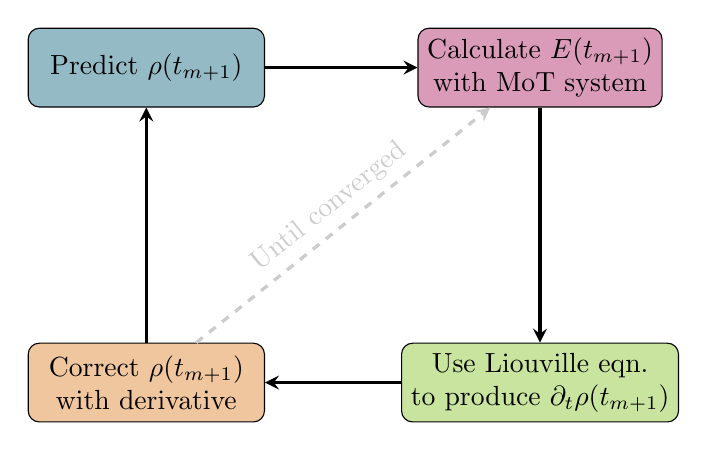
\begin{tikzpicture}[node distance=4cm]

\node (predict) [step1] {Predict $\rho(t_{m + 1})$};
\node (mot) [step2, right of=predict, xshift=1cm] {Calculate $\vb{E}(t_{m + 1})$ \\ with MoT system};
\node (evaluate) [step3, below of=mot] {Use Liouville eqn.\ \\ to produce $\partial_t \rho(t_{m + 1})$};
\node (correct) [step4, below of=predict] {Correct $\rho(t_{m + 1})$ \\ with derivative};

\draw [arrow] (predict) -- (mot);
\draw [arrow] (mot) -- (evaluate);
\draw [arrow] (evaluate) -- (correct);
\draw [arrow] (correct) -- (predict) node [midway, above, sloped] (n1) {};
\draw [gray!40, dashed, arrow] (correct) -- (mot) node [midway, above, sloped] (n2) {Until converged};

\end{tikzpicture}
